\documentclass[aspectratio=169]{beamer}

% ===================== PAQUETES =====================
\usepackage{iftex}
\ifPDFTeX
  \usepackage[utf8]{inputenc}
  \usepackage[T1]{fontenc}
  \usepackage{lmodern}
\else
  \usepackage{fontspec}
\fi
\usepackage[spanish,es-noshorthands]{babel}
\usepackage{graphicx}
\usepackage{booktabs}
\usepackage{xcolor}
\usepackage{amsmath,amssymb}
\usepackage{array}
\usepackage{tikz}
\usepackage{hyperref}
\usetikzlibrary{positioning,arrows.meta}

% Figuras: las genera figuras_presentacion.py con el codigo de Ejercicio_1/codigo y Ejercicio_2/codigo.
% Numeros citados: resultados.json (mismo script).
\graphicspath{{figs/}}

% ===================== COLORES =====================
\definecolor{itbaBlue}{RGB}{2, 86, 138}
\definecolor{itbaGray}{RGB}{200, 200, 200}
\definecolor{itbaGold}{RGB}{255, 215, 0}
\definecolor{itbaRed}{RGB}{204, 0, 0}
\definecolor{softGray}{RGB}{120, 120, 120}

% ===================== TEMA =====================
\usetheme{default}
\setbeamercolor{title}{fg=white, bg=itbaBlue}
\setbeamercolor{frametitle}{fg=white, bg=itbaBlue}
\setbeamercolor{structure}{fg=itbaBlue}
\setbeamercolor{block title}{fg=white, bg=itbaBlue}
\setbeamercolor{block body}{fg=black, bg=itbaGray!20}
\setbeamercolor{block title alerted}{fg=black, bg=itbaGold}
\setbeamercolor{block body alerted}{fg=black, bg=itbaGray!30}
\setbeamertemplate{navigation symbols}{}
\setbeamertemplate{blocks}[rounded][shadow=false]
\setbeamertemplate{itemize items}[triangle]
\setbeamerfont{frametitle}{size=\large,series=\bfseries}
\setbeamerfont{title}{size=\Large,series=\bfseries}
\setbeamertemplate{footline}{%
  \begin{beamercolorbox}[wd=\paperwidth,ht=0.6cm,dp=0cm]{}%
    \hspace{1em}{\tiny\color{softGray}\insertsectionhead}\hfill
    \raisebox{0.12cm}{\logoitba{0.05\paperwidth}}\hspace{0.6em}%
    \raisebox{0.17cm}{\tiny\color{softGray}\insertframenumber\,/\,\inserttotalframenumber}\hspace{1em}%
  \end{beamercolorbox}}

\newcommand{\bignum}[3][itbaBlue]{%
  \begin{minipage}[t]{\linewidth}\centering
    {\fontsize{28}{30}\selectfont\bfseries\color{#1}#2}\\[0.25em]
    {\footnotesize #3}
  \end{minipage}}
\newcommand{\clave}[1]{%
  \vfill
  \begin{alertblock}{Clave}\footnotesize #1\end{alertblock}}
\newcommand{\fuente}[1]{{\tiny\color{softGray}#1}}
\newcommand{\figslide}[3]{%
  \begin{frame}{#1}
    \centering
    \includegraphics[width=0.97\textwidth, height=0.74\textheight, keepaspectratio]{#2}\\[-0.1em]
    {\scriptsize #3}
  \end{frame}}
\newcommand{\logoitba}[1]{\IfFileExists{figs/itba_logo.png}{
\includegraphics[width=#1]{itba_logo.png}}{}}

% ===================== METADATOS =====================
\title{Deep Learning: Autoencoders y Autoencoders Variacionales}
\subtitle{TP5: Autoencoder y Denoising Autoencoder sobre letras; VAE sobre sprites de Pok\'emon}
\author{Britez, Santiago \and Kantor, Marcos \and S\'anchez Toledo, Mariano \\[0.2em]
\small Sistemas de Inteligencia Artificial --- TP5}
\institute{Instituto Tecnol\'ogico de Buenos Aires}
\date{2026}

\begin{document}

% ====================================================================== 1
\begin{frame}[plain]
  \begin{center}\vspace{0.2cm}\logoitba{0.22\textwidth}\end{center}
  \vspace{-0.4cm}
  \titlepage
\end{frame}

% ====================================================================== 2
\section{Introducci\'on}

\begin{frame}{Dos ejercicios, una pregunta: ?`qu\'e hace \'util a un espacio latente?}
  \begin{columns}[T,onlytextwidth]
    \column{0.48\textwidth}
      \begin{block}{Ej.\ 1 --- Autoencoder con letras (7$\times$5)}
        \footnotesize
        Representar 32 letras con \textbf{2 n\'umeros reales} y recuperarlas con $\le 1$ p\'ixel mal; despu\'es, quitar ruido (\emph{denoising}).
      \end{block}
      \vspace{0.25cm}
      \bignum{0 px}{de error en las 32 letras con el modelo final \\ (un PCA con 2 componentes deja hasta 15 px)}
    \column{0.48\textwidth}
      \begin{block}{Ej.\ 2 --- VAE con sprites de Pok\'emon (32$\times$32 RGB)}
        \footnotesize
        El autoencoder reconstruye, pero su espacio latente tiene \textbf{huecos}. El t\'ermino KL del VAE lo vuelve \textbf{muestreable} y permite generar.
      \end{block}
      \vspace{0.25cm}
      \bignum{6,8 vs.\ 19,1}{distancia de Fr\'echet de las muestras del prior al conjunto: VAE vs.\ autoencoder ($d$=32, 3 semillas). Piso con Pok\'emon reales no vistos: 4,1}
  \end{columns}
  \vfill
  \centering\fuente{Objetivos: (1) qu\'e arquitectura y optimizador permiten comprimir; (2) qu\'e aporta entrenar con ruido; (3) qu\'e cambia el esquema variacional; (4) generar una muestra nueva y justificar que pertenece al conjunto.}
\end{frame}

% ====================================================================== 3
\begin{frame}{Todo el aprendizaje est\'a escrito desde cero en \texttt{numpy} y validado}
  \begin{columns}[T,onlytextwidth]
    \column{0.54\textwidth}
      \begin{block}{Implementaci\'on propia}
        \footnotesize
        \begin{itemize}
          \item Capas densas y retropropagaci\'on a mano.
          \item Optimizadores SGD, Momentum y Adam.
          \item Autoencoder, Denoising AE y VAE (reparametrizaci\'on, KL cerrada, factor $\beta$).
          \item M\'etricas: error en p\'ixeles y distancia de Fr\'echet.
        \end{itemize}
      \end{block}
      \begin{block}{Bibliotecas de soporte (no resuelven el TP)}
        \footnotesize
        \texttt{numpy}: \'algebra matricial (incluida la SVD). \texttt{PIL}: leer y escalar im\'agenes. \texttt{matplotlib}, \texttt{pandas}: gr\'aficos y tablas.
      \end{block}
    \column{0.42\textwidth}
      \bignum{$\sim\!10^{-8}$}{error relativo del gradiente anal\'itico frente a diferencias finitas \\ (AE: $8{,}8\cdot10^{-9}$; VAE: $1{,}8\cdot10^{-8}$)}


      \vspace{0.3cm}
      {\footnotesize Semillas fijas y varias por configuraci\'on (5 en el Ej.\ 1, 3 en el Ej.\ 2); hiperpar\'ametros en \texttt{config.json}.}
  \end{columns}
  \clave{El objetivo es \textbf{entender qu\'e controla la representaci\'on}: arquitectura, optimizador, ruido y t\'ermino variacional.}
\end{frame}

% ====================================================================== 4
\section{Ej. 1a: Autoencoder}

\begin{frame}{Ej.\ 1a: 32 letras de 35 p\'ixeles deben caber en un plano de 2 dimensiones}
  \begin{columns}[T,onlytextwidth]
    \column{0.60\textwidth}
      \centering
      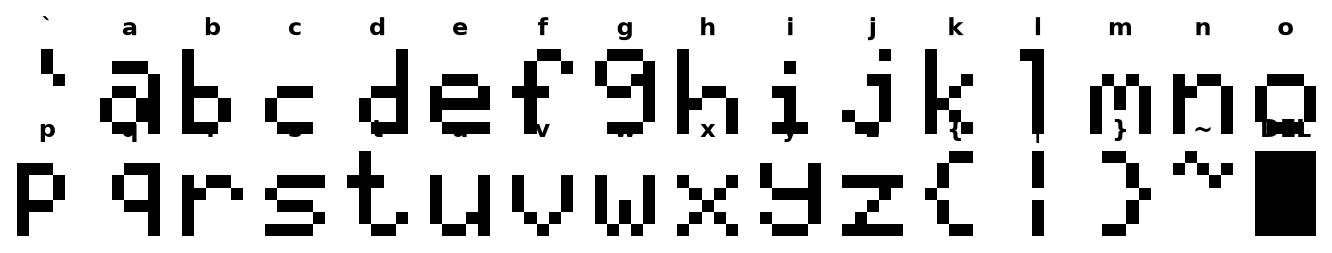
\includegraphics[width=\textwidth]{f_letras.png}
      \\[-0.2em]\fuente{\texttt{font.h} de la c\'atedra: 32 patrones binarios de 7$\times$5 (0x60--0x7f).}
    \column{0.38\textwidth}
      \footnotesize
      \begin{block}{Informaci\'on vs.\ optimizaci\'on}
        32 patrones requieren $\log_2 32 = 5$ bits: dos reales alcanzan de sobra.
        La dificultad es que el decodificador \textbf{dibuje 32 islas} y que el descenso por gradiente las encuentre.
      \end{block}
      \begin{block}{Criterio de \'exito del enunciado}
        Peor patr\'on con $\le 1$ p\'ixel incorrecto tras umbralizar $\hat{x}>0{,}5$.
      \end{block}
  \end{columns}
\end{frame}

% ====================================================================== 5
\begin{frame}{Arquitectura: cuello de botella lineal de 2 unidades y entrop\'ia cruzada}
  \centering
  \begin{tikzpicture}[x=1cm,y=1cm,
     capa/.style={draw=itbaBlue,fill=itbaGray!25,rounded corners=2pt,minimum height=2.4cm,minimum width=0.75cm,font=\scriptsize,align=center},
     flecha/.style={-{Latex[length=1.6mm]},draw=softGray}]
    \node[capa] (a) at (0,0) {35};
    \node[capa,minimum height=1.9cm] (b) at (2.1,0) {32};
    \node[capa,minimum height=1.3cm] (c) at (4.2,0) {16};
    \node[capa,fill=itbaGold,minimum height=0.6cm] (z) at (6.3,0) {$z$\\2};
    \node[capa,minimum height=1.3cm] (d) at (8.4,0) {16};
    \node[capa,minimum height=1.9cm] (e) at (10.5,0) {32};
    \node[capa] (f) at (12.6,0) {35};
    \foreach \u/\v in {a/b,b/c,c/z,z/d,d/e,e/f} \draw[flecha] (\u) -- (\v);
    \node[font=\scriptsize,itbaBlue] at (3.15,-1.85) {codificador $f_\theta$ ($\tanh$)};
    \node[font=\scriptsize,itbaBlue] at (9.45,-1.85) {decodificador $g_\phi$ ($\tanh$ + sigmoide)};
    \node[font=\scriptsize,itbaRed] at (6.3,1.2) {cuello de botella lineal};
  \end{tikzpicture}
  \vspace{0.3cm}
  \begin{columns}[T,onlytextwidth]
    \column{0.48\textwidth}
      \footnotesize
      \begin{block}{P\'erdida}
        {\scriptsize\[ \mathcal{L}=-\sum_i \big[x_i\log\hat{x}_i+(1-x_i)\log(1-\hat{x}_i)\big] \]}
      \end{block}
    \column{0.48\textwidth}
      \footnotesize
      \begin{block}{Por qu\'e entrop\'ia cruzada binaria}
        Los p\'ixeles son 0/1. El gradiente respecto del logit, $\partial\mathcal{L}/\partial a_i=\hat{x}_i-x_i$, no lleva el factor $\sigma'(a)$: la red sigue aprendiendo aunque se equivoque con confianza (con error cuadr\'atico + sigmoide se estanca).
      \end{block}
  \end{columns}
\end{frame}

% ====================================================================== 6
\figslide{Una capa oculta no alcanza; con dos, Adam llega en las 5 semillas}{f_1a_exito.png}{\fuente{5 semillas por barra; 3000 \'epocas \emph{full-batch}; SGD ($\eta$=0,03), Momentum (0,005), Adam (0,005). Misma escala en ambos paneles. Con dos capas ocultas Adam necesita una mediana de 200--500 \'epocas; Momentum, 2 a 5 veces m\'as.}}

% ====================================================================== 7
\begin{frame}{El modelo final recupera las 32 letras sin errores; el PCA lineal no puede}
  \centering
  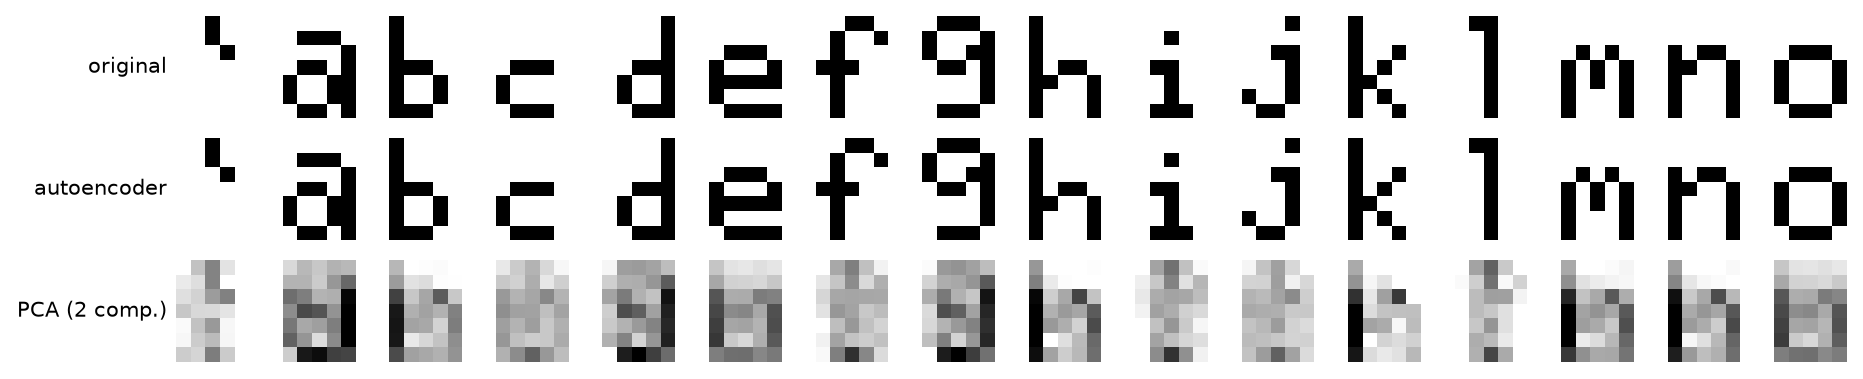
\includegraphics[width=0.96\textwidth,height=0.38\textheight,keepaspectratio]{f_1a_recon.png}\\[0.2em]
  \begin{columns}[T,onlytextwidth]
    \column{0.30\textwidth}\bignum{0 px}{peor patr\'on, autoencoder \\ ($\le 1$ px desde la \'epoca 450)}
    \column{0.30\textwidth}\bignum[itbaRed]{15 px}{peor patr\'on, PCA 2 comp. \\ (7,2 en promedio)}
    \column{0.36\textwidth}\footnotesize 35--32--16--2 \texttt{tanh}, Adam $\eta=5\cdot10^{-3}$, 6000 \'epocas, semilla 0. La no linealidad es lo que permite que 2 dimensiones alcancen.
  \end{columns}
  \clave{Un autoencoder lineal converge a PCA (teorema visto en clase; Baldi \& Hornik, 1989): lo que aporta el modelo no lineal es una \textbf{variedad curva} en lugar de un plano.}
\end{frame}

% ====================================================================== 8
\begin{frame}{El espacio latente 2-D ubica las 32 letras, pero entre ellas quedan huecos}
  \centering
  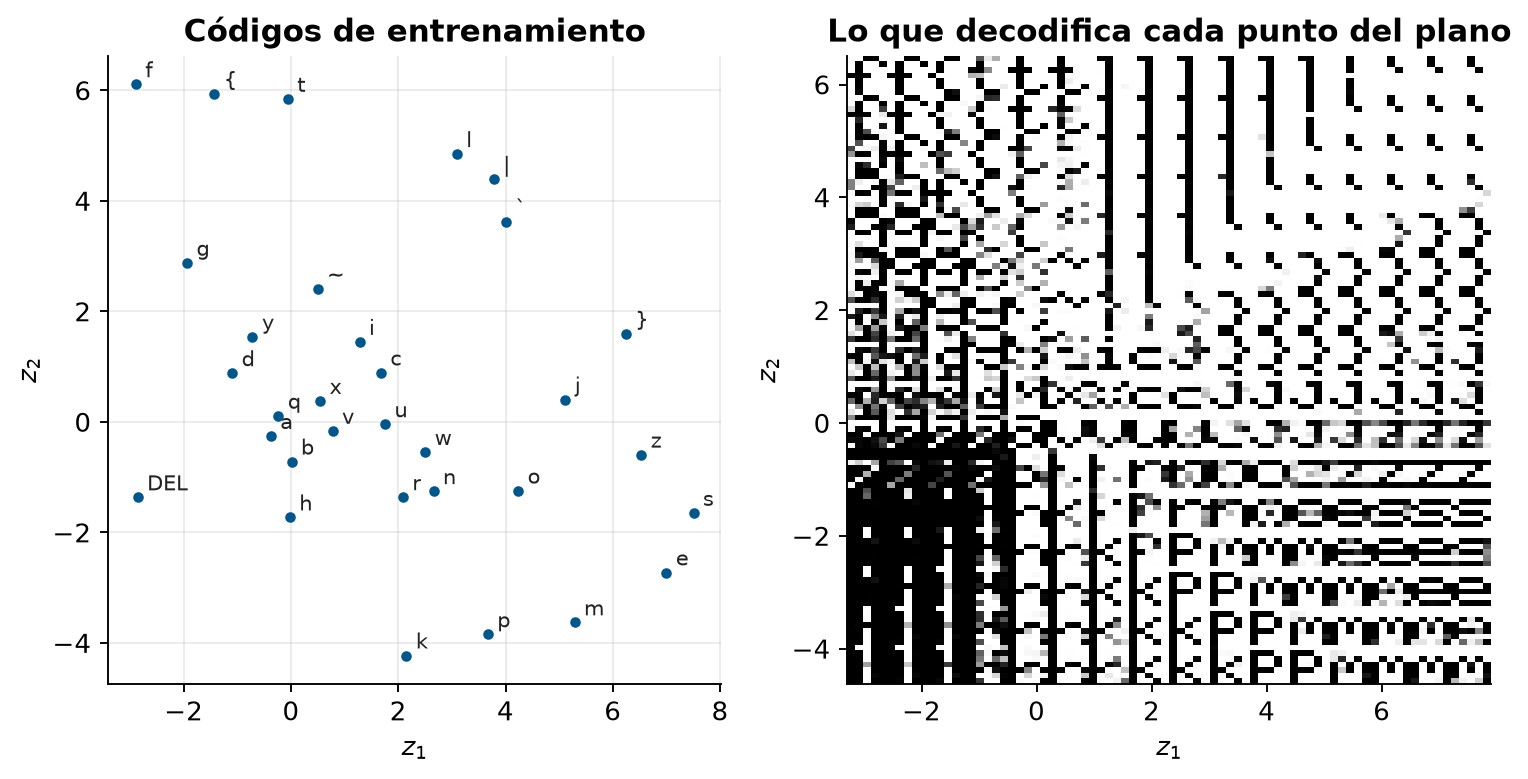
\includegraphics[width=0.93\textwidth,height=0.70\textheight,keepaspectratio]{f_1a_atlas.png}\\[-0.1em]
  {\scriptsize Izquierda: los 32 c\'odigos (entre $-4{,}2$ y $7{,}5$). Derecha: lo que decodifica cada punto de una grilla del plano. Cerca de un c\'odigo se ve su letra; entre c\'odigos aparecen mezclas e im\'agenes sin sentido. \textbf{Nada en la p\'erdida ordena este espacio.}}
\end{frame}

% ====================================================================== 9
\begin{frame}{Decodificar un punto intermedio genera una letra nueva: una mezcla de sus vecinas}
  \centering
  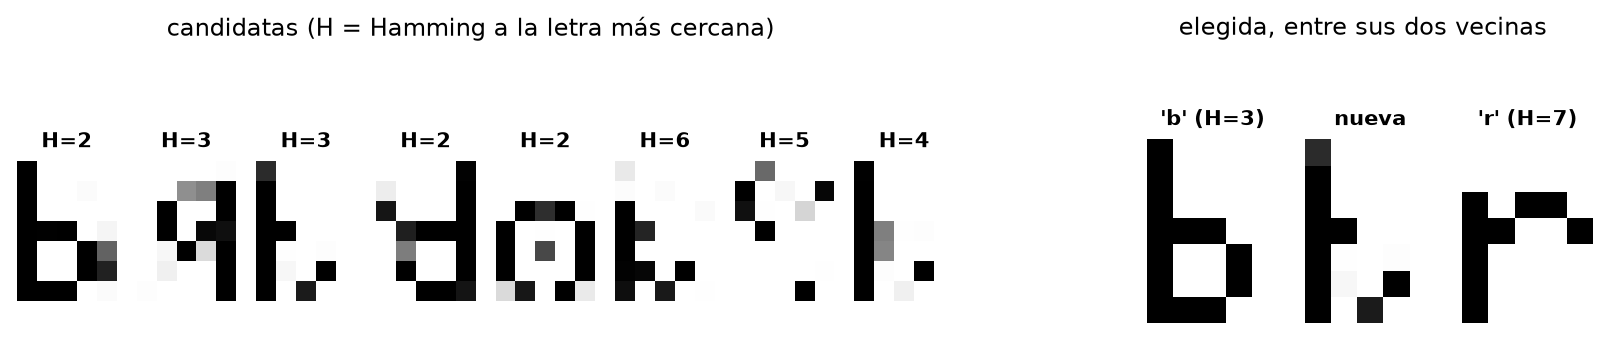
\includegraphics[width=0.92\textwidth,height=0.40\textheight,keepaspectratio]{f_1a_nuevas.png}\\[0.2em]
  \begin{columns}[T,onlytextwidth]
    \column{0.5\textwidth}
      \footnotesize
      \begin{block}{C\'omo se elige}
        Grilla de 41$\times$41 puntos en el rango de los c\'odigos. Se retienen las im\'agenes (i) a distancia de Hamming $\ge 2$ de \textbf{toda} letra de entrenamiento y (ii) n\'itidas ($\le 2$ p\'ixeles grises): 171 de 1681.
      \end{block}
    \column{0.46\textwidth}
      \footnotesize
      \begin{block}{Qu\'e significa ``nueva''}
        La elegida ($z=(0{,}35;\,-0{,}73)$) est\'a a 3 p\'ixeles de la ``b'' y a 7 de la ``r''. No es una letra del alfabeto: es una \textbf{interpolaci\'on}. Que ``parezca una letra'' es un juicio humano.
      \end{block}
  \end{columns}
\end{frame}

% ====================================================================== 10
\section{Ej. 1b: Denoising Autoencoder}

\begin{frame}{Ej.\ 1b: se entrena con la entrada corrupta y se exige reconstruir la limpia}
  \begin{columns}[T,onlytextwidth]
    \column{0.52\textwidth}
      \footnotesize
      \begin{block}{Dise\~no del experimento}
        \begin{itemize}
          \item Ruido: cada p\'ixel se invierte con probabilidad $p$ (sal y pimienta sobre im\'agenes binarias).
          \item Entrada ruidosa $\tilde{x}$, \textbf{objetivo limpio} $x$:\; $\mathcal{L}\big(x,\,g_\phi(f_\theta(\tilde{x}))\big)$.
          \item Ruido \textbf{nuevo en cada \'epoca}: con 32 patrones, un ruido fijo se memorizar\'ia.
          \item Misma arquitectura del 1a (35--32--16--$d$), $d\in\{2,8\}$, $p_{train}\in\{0;\,0{,}05;\,0{,}1;\,0{,}2\}$, 5 semillas.
        \end{itemize}
      \end{block}
    \column{0.44\textwidth}
      \begin{block}{Por qu\'e la misma arquitectura}
        \footnotesize
        Para aislar el efecto del ruido. $d=8$ permite comparar con un cuello de botella menos estrecho.
      \end{block}
      \vspace{0.2cm}
      \bignum[itbaRed]{0,9 $\to$ 3,3 px}{con 2,5\,\% de ruido, el autoencoder entrenado sin ruido ($d$=2) \emph{agrega} errores}
  \end{columns}
\end{frame}

% ====================================================================== 11
\figslide{Con $d=8$ el DAE deja 0,44 px donde la entrada ten\'ia 3,5}{f_1b_curvas.png}{\fuente{Media $\pm$ desv\'io entre 5 semillas; 32 letras $\times$ 20 muestras de ruido por punto; semillas de ruido de evaluaci\'on distintas de las de entrenamiento. Misma escala vertical. L\'inea roja punteada: error de la entrada sin red ($35\,p$).}}

% ====================================================================== 12
\begin{frame}{El DAE devuelve letras v\'alidas; con demasiado ruido, la letra equivocada}
  \centering
  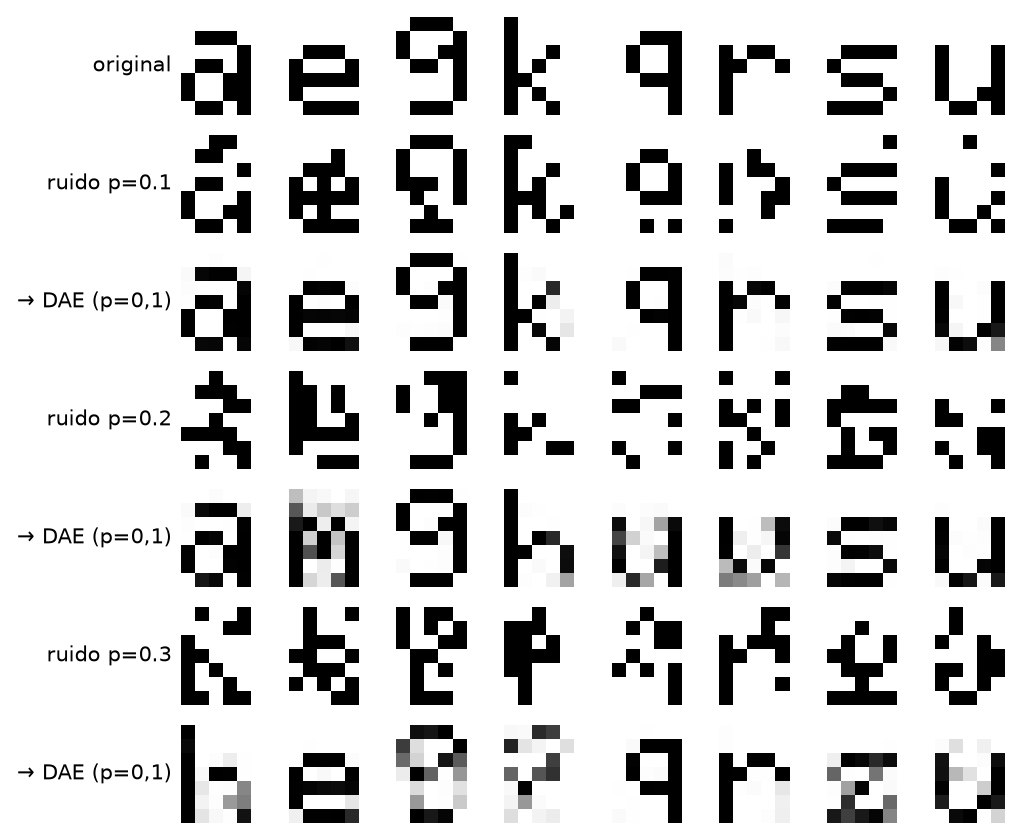
\includegraphics[width=0.74\textwidth,height=0.52\textheight,keepaspectratio]{f_1b_ejemplos.png}\\[0.1em]
  {\scriptsize DAE $d$=8 entrenado con $p$=0,1 (semilla 0). Con $p$=0,3 la entrada queda m\'as cerca de otra letra: error \emph{confiado}, an\'alogo a los estados espurios de Hopfield (TP4).}
  \clave{El ruido de entrenamiento es un compromiso: protege a niveles altos pero cuesta precisi\'on sin ruido ($d$=2, $p_{train}$=0,2: 1,8 px aun con la entrada limpia; con $d$=8, 0,09).}
\end{frame}

% ====================================================================== 13
\section{Ej. 2: VAE con Pok\'emon}

\begin{frame}{Ej.\ 2: un conjunto nuevo y m\'as exigente, 809 sprites de Pok\'emon}
  \centering
  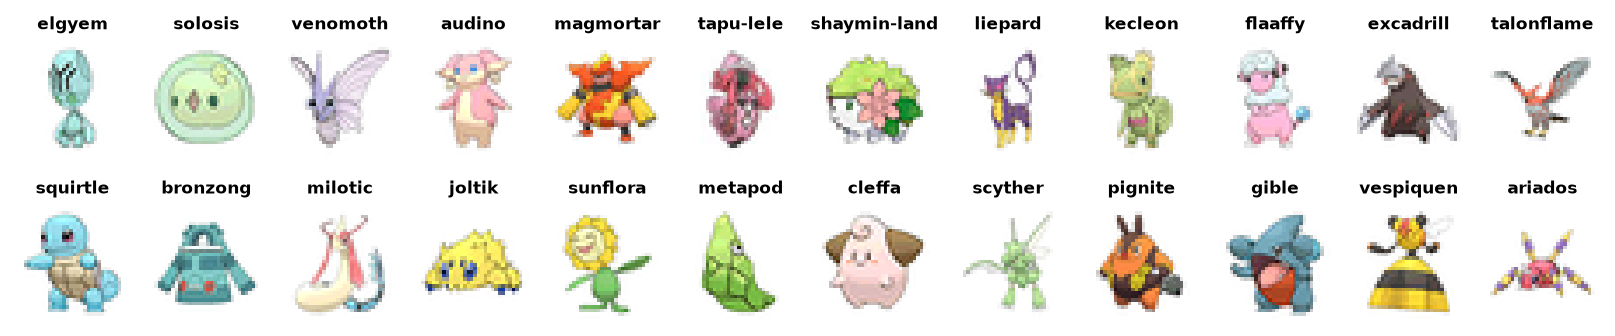
\includegraphics[width=0.90\textwidth,height=0.34\textheight,keepaspectratio]{f_2_dataset.png}\\[0.2em]
  \begin{columns}[T,onlytextwidth]
    \column{0.49\textwidth}
      \footnotesize
      \begin{block}{Por qu\'e este conjunto}
        \begin{itemize}
          \item \textbf{Sin clases}: cada Pok\'emon aparece una vez; no hay prototipos que memorizar.
          \item \textbf{En color}: 3 canales, el modelo tambi\'en aprende paletas.
          \item Criterio claro de \'exito al generar: que no sea ninguno de los 809 y que igual parezca un Pok\'emon.
        \end{itemize}
      \end{block}
    \column{0.48\textwidth}
      \footnotesize
      \begin{block}{Preprocesamiento y partici\'on}
        \begin{itemize}
          \item Composici\'on sobre fondo blanco, recorte a la figura, centrado con 6\,\% de margen.
          \item Escalado a 32$\times$32 RGB: 3072 valores en $[0,1]$.
          \item \textbf{81 Pok\'emon completos (10\,\%) retenidos}; los 728 restantes se duplican con su reflejo horizontal (1456 im\'agenes).
        \end{itemize}
      \end{block}
  \end{columns}
\end{frame}

% ====================================================================== 14
\begin{frame}{La red base es la del Ej.\ 1 a otra escala; cada decisi\'on se tom\'o midiendo}
  \begin{columns}[T,onlytextwidth]
    \column{0.56\textwidth}
      \footnotesize
      \begin{block}{Arquitectura e hiperpar\'ametros}
        \begin{itemize}
          \item Codificador 3072--512--256--$d$; decodificador sim\'etrico con salida sigmoide.
          \item \textbf{ReLU en lugar de tanh}: con 3072 entradas tanh satura (prueba preliminar: BCE de entrenamiento 888 vs.\ 701 nats).
          \item Adam, $\eta=3\cdot10^{-4}$, lotes de 64, 300 \'epocas. Con $\eta=10^{-3}$ sobreajusta.
          \item $d\in\{2,\,32\}$: con 2 el espacio se puede \textbf{ver}; con 32 se puede \textbf{dibujar}.
        \end{itemize}
      \end{block}
    \column{0.41\textwidth}
      \begin{block}{BCE con p\'ixeles continuos}
        \footnotesize
        Su m\'inimo no es 0 sino la entrop\'ia de los propios p\'ixeles: se compara contra un piso y un techo.
      \end{block}
      \vspace{0.15cm}
      \bignum{600 -- 981}{nats por imagen: reconstrucci\'on perfecta vs.\ predecir siempre la imagen media (Pok\'emon no vistos)}
  \end{columns}
  \clave{El autoencoder del Ej.\ 1 no dice \textbf{d\'onde} quedan los c\'odigos: para generar no sabemos de qu\'e distribuci\'on sacar $z$. Eso es lo que resuelve el esquema variacional.}
\end{frame}

% ====================================================================== 15
\begin{frame}{VAE: el codificador devuelve una distribuci\'on y la p\'erdida suma un regularizador}
  \begin{columns}[T,onlytextwidth]
    \column{0.56\textwidth}
      \begin{block}{Modelo generativo e inferencia variacional}
        \footnotesize
        $z\sim p(z)=\mathcal{N}(0,I)$, \quad $x\mid z\sim p_\phi(x\mid z)$ (Bernoulli por p\'ixel).\\[0.2em]
        $p(z\mid x)$ es intratable: se aproxima con $q_\theta(z\mid x)=\mathcal{N}\big(\mu_\theta(x),\mathrm{diag}\,\sigma^2_\theta(x)\big)$.
      \end{block}
      \footnotesize
      \[ \log p(x)=\mathrm{KL}\big(q(z|x)\,\|\,p(z|x)\big)+\mathcal{L}\;\;\Rightarrow\;\;\mathcal{L}\le\log p(x) \]
      \[ -\mathcal{L}=\underbrace{-\mathbb{E}_{q}\big[\log p_\phi(x|z)\big]}_{\text{reconstrucci\'on (BCE)}}+\underbrace{\mathrm{KL}\big(q_\theta(z|x)\,\|\,\mathcal{N}(0,I)\big)}_{\text{regularizador}} \]
    \column{0.40\textwidth}
      \footnotesize
      \begin{block}{Qu\'e hace cada t\'ermino}
        \textbf{Reconstrucci\'on}: cada $z$ muestreado debe decodificar en algo parecido a $x$.\\[0.3em]
        \textbf{KL}: empuja cada $q(z|x)$ hacia el prior; los c\'odigos cubren $\mathcal{N}(0,I)$ sin huecos.
      \end{block}
      \begin{block}{Factor $\beta$ (Higgins et al., 2017)}
        P\'erdida $=\mathrm{BCE}+\beta\cdot\mathrm{KL}$. $\beta=1$: cota variacional. $\beta=0$: sin regularizador, se comporta como el autoencoder del Ej.\ 1.
      \end{block}
  \end{columns}
\end{frame}

% ====================================================================== 16
\begin{frame}{La reparametrizaci\'on permite retropropagar a trav\'es del muestreo}
  \begin{columns}[T,onlytextwidth]
    \column{0.50\textwidth}
      \centering
      \begin{tikzpicture}[x=0.92cm,y=0.85cm,
         caja/.style={draw=itbaBlue,fill=itbaGray!25,rounded corners=2pt,minimum height=0.75cm,minimum width=1.25cm,font=\scriptsize,align=center},
         flecha/.style={-{Latex[length=1.6mm]},draw=softGray}]
        \node[caja] (x) at (0,0) {$x$\\3072};
        \node[caja] (h) at (1.9,0) {512--256\\ReLU};
        \node[caja] (mu) at (3.9,0.75) {$\mu$};
        \node[caja] (lv) at (3.9,-0.75) {$\log\sigma^2$};
        \node[caja,fill=itbaGold] (z) at (5.9,0) {$z=\mu+\sigma\odot\varepsilon$};
        \node[font=\scriptsize,itbaRed] (e) at (5.9,1.35) {$\varepsilon\sim\mathcal{N}(0,I)$};
        \node[caja] (d) at (5.9,-1.7) {256--512\\ReLU};
        \node[caja] (o) at (3.4,-1.7) {$\hat{x}$\\sigmoide};
        \draw[flecha] (x)--(h); \draw[flecha] (h)--(mu); \draw[flecha] (h)--(lv);
        \draw[flecha] (mu)--(z); \draw[flecha] (lv)--(z); \draw[flecha,draw=itbaRed] (e)--(z);
        \draw[flecha] (z)--(d); \draw[flecha] (d)--(o);
      \end{tikzpicture}
      \\[0.3em]\fuente{El azar entra por $\varepsilon$; $\mu$ y $\sigma$ quedan en un camino derivable.}
    \column{0.47\textwidth}
      \scriptsize
      \begin{block}{KL en forma cerrada (gaussianas diagonales)}
        $\mathrm{KL}=\tfrac12\sum_{j=1}^{d}\big(\mu_j^2+\sigma_j^2-\log\sigma_j^2-1\big)$
      \end{block}
      \begin{block}{Gradientes que llegan al codificador}
        $\partial\mathcal{L}/\partial\mu=\delta_z+\beta\mu$\\[0.3em]
        $\partial\mathcal{L}/\partial\log\sigma^2=\tfrac12\,\delta_z\odot\varepsilon\odot\sigma+\tfrac{\beta}{2}(\sigma^2-1)$\\[0.3em]
        $\delta_z$: error de reconstrucci\'on retropropagado por el decodificador.
      \end{block}
  \end{columns}
  \clave{El decodificador s\'olo recibe gradiente de reconstrucci\'on; el codificador, reconstrucci\'on m\'as KL. Verificado con diferencias finitas fijando $\varepsilon$.}
\end{frame}

% ====================================================================== 17
\begin{frame}{?`C\'omo medir que una muestra ``pertenece'' al conjunto si no hay etiquetas?}
  \begin{columns}[T,onlytextwidth]
    \column{0.50\textwidth}
      \footnotesize
      \begin{block}{Distancia de Fr\'echet entre distribuciones}
        Se ajusta una gaussiana a cada nube de rasgos y se calcula
        \[ \|m_1-m_2\|^2+\mathrm{tr}\big(S_1+S_2-2\,(S_1S_2)^{1/2}\big) \]
        Es la idea del FID (Heusel et al., 2017). Rasgos: las 20 primeras componentes principales del entrenamiento (SVD de \texttt{numpy}).
      \end{block}
    \column{0.47\textwidth}
      \footnotesize
      \begin{block}{Un piso para interpretarla}
        La misma distancia para los \textbf{81 Pok\'emon reales no vistos}, con igual tama\~no de muestra: \textbf{4,1}. Si las muestras generadas se acercan al piso, se parecen al conjunto tanto como un Pok\'emon real nuevo.
      \end{block}
      \begin{block}{Fracci\'on de casi copias}
        Muestras m\'as cerca de un dato de entrenamiento que la mitad de la distancia t\'ipica de un Pok\'emon nuevo. Una copia no es una muestra nueva.
      \end{block}
  \end{columns}
  \clave{No se eval\'ua una imagen suelta sino la \textbf{distribuci\'on} de 2000 muestras de $z\sim\mathcal{N}(0,I)$, siempre contra una referencia de datos reales.}
\end{frame}

% ====================================================================== 18
\figslide{El KL cuesta algo de reconstrucci\'on, pero acerca las muestras al conjunto real}{f_2_beta.png}{\fuente{24 redes: $\beta\in\{0;\,0{,}25;\,1;\,4\}\times d\in\{2;\,32\}\times$ 3 semillas (barras de error = desv\'io). Con $d$=32: BCE 802 $\to$ 815 nats, KL 299 $\to$ 37 nats, Fr\'echet 19,1 $\to$ 6,8 al pasar de $\beta$=0 a $\beta$=1. $\beta$=4 no mejora las muestras (7,4) y eleva las casi copias de 1\,\% a 9\,\%.}}

% ====================================================================== 19
\begin{frame}{En 2 dimensiones el VAE ordena el espacio por color y silueta, sin etiquetas}
  \centering
  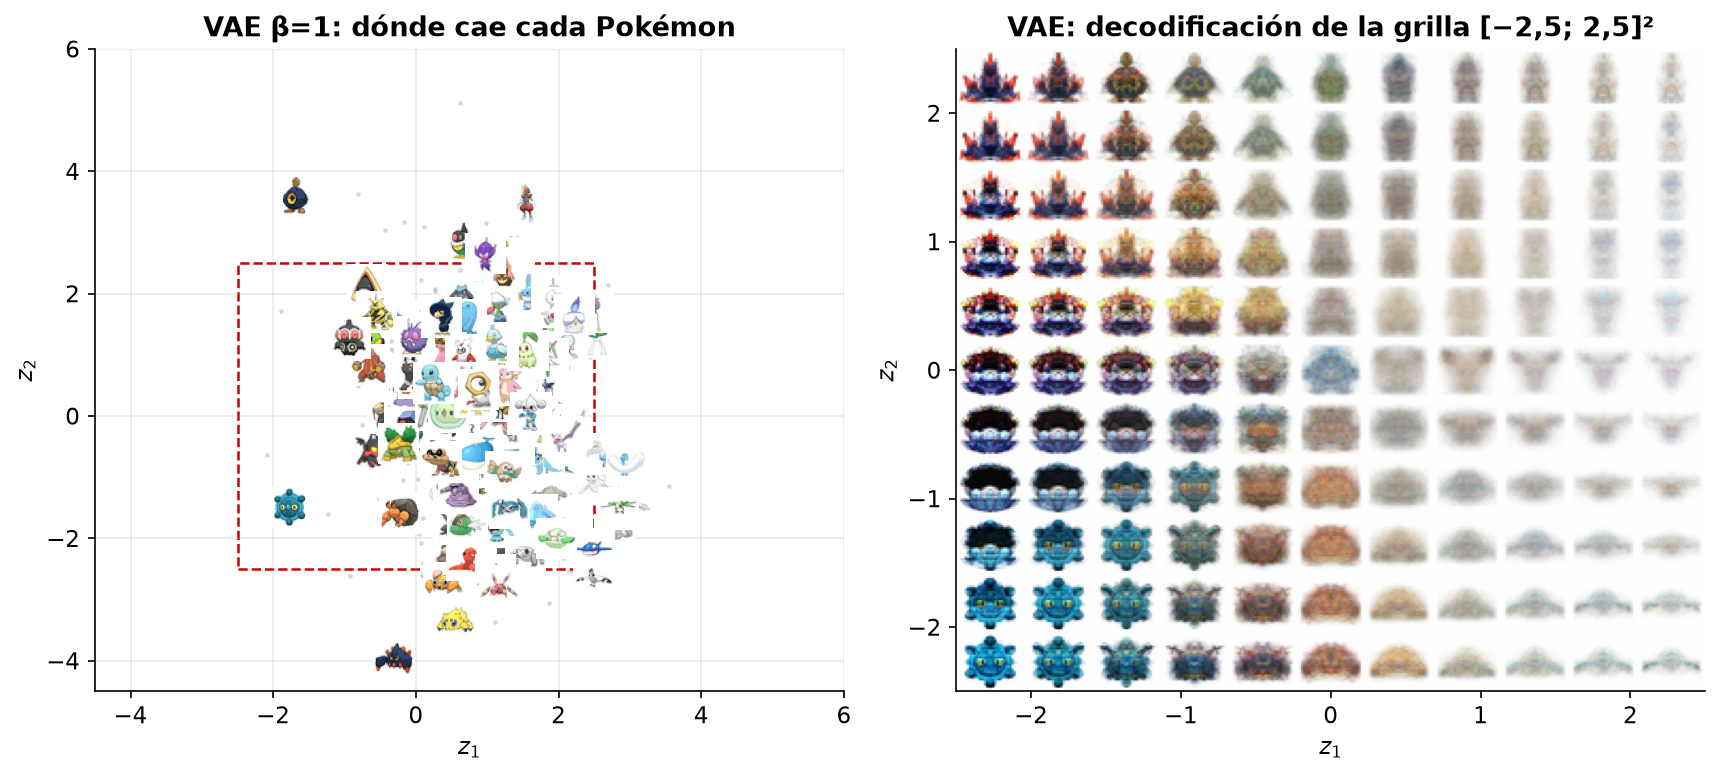
\includegraphics[width=0.90\textwidth,height=0.70\textheight,keepaspectratio]{f_2_latente.png}\\[-0.1em]
  {\scriptsize VAE $\beta$=1, $d$=2, semilla 0. Izquierda: media posterior $\mu$ de cada Pok\'emon de entrenamiento (cuadro rojo: $[-2{,}5;\,2{,}5]^2$, donde cae el 92\,\% de los c\'odigos; con $\beta$=0, el 74\,\%). Derecha: decodificaci\'on de la grilla. Transiciones suaves, pero im\'agenes borrosas: $d$=2 sirve para ver, no para dibujar.}
\end{frame}

% ====================================================================== 20
\begin{frame}{Con las mismas $z\sim\mathcal{N}(0,I)$, el autoencoder da ruido y el VAE, figuras}
  \centering
  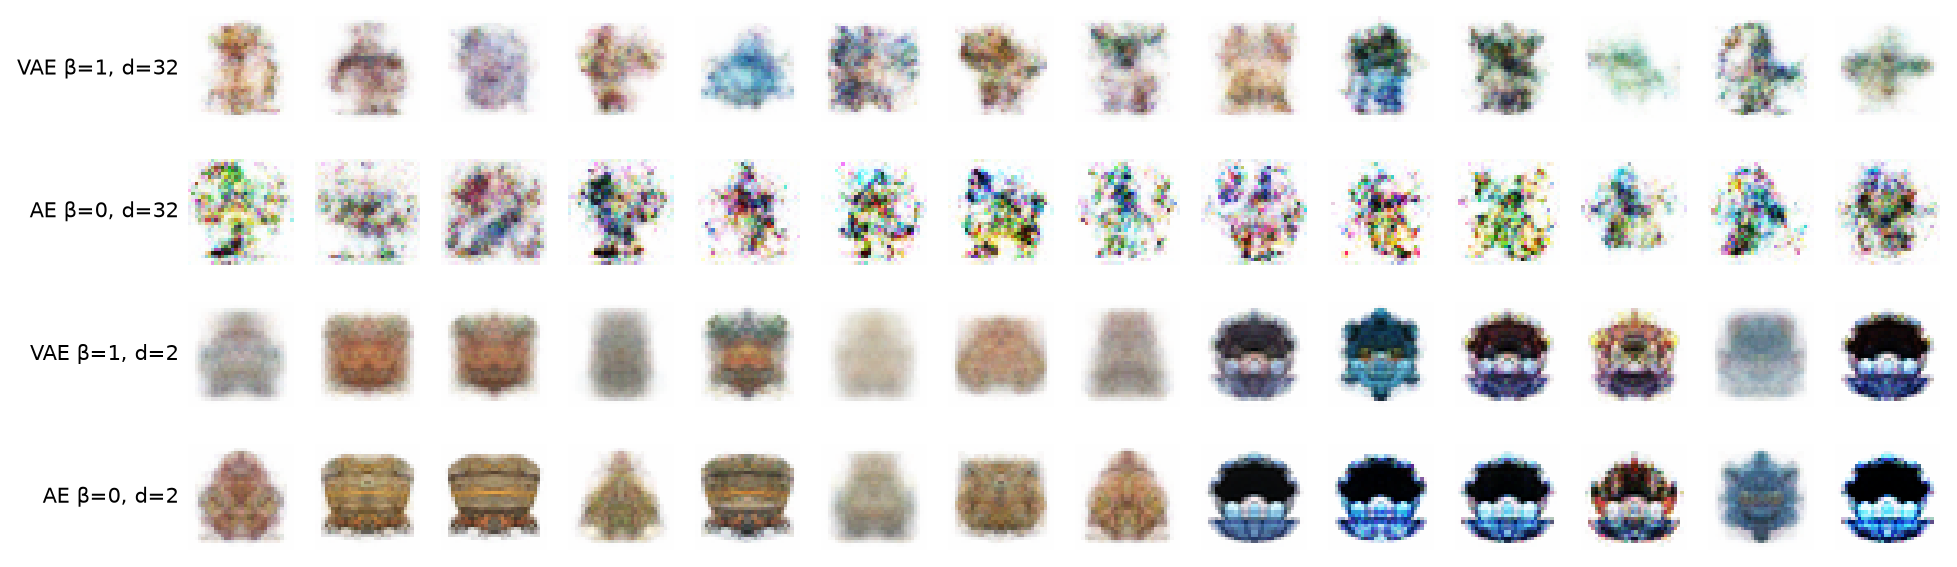
\includegraphics[width=0.94\textwidth,height=0.60\textheight,keepaspectratio]{f_2_prior.png}\\[0.1em]
  \begin{columns}[T,onlytextwidth]
    \column{0.31\textwidth}\bignum{7,4}{Fr\'echet, VAE $d$=32 \\ (semilla 0; piso 4,1)}
    \column{0.31\textwidth}\bignum[itbaRed]{18,6}{Fr\'echet, AE $d$=32 \\ (semilla 0)}
    \column{0.34\textwidth}\footnotesize\vspace{0.1cm}Los c\'odigos del AE tienen desv\'io $\approx 2{,}6$ y 299 nats de KL: el prior cae en zonas que su decodificador nunca vio. Son los \textbf{huecos} del Ej.\ 1, ahora en 32 dimensiones.
  \end{columns}
\end{frame}

% ====================================================================== 21
\begin{frame}{Un Pok\'emon nuevo: no es copia y est\'a tan cerca del conjunto como uno real}
  \begin{columns}[T,onlytextwidth]
    \column{0.52\textwidth}
      \centering
      
\includegraphics[width=0.86\textwidth]{f_2_elegida.png}\\[0.2em]
      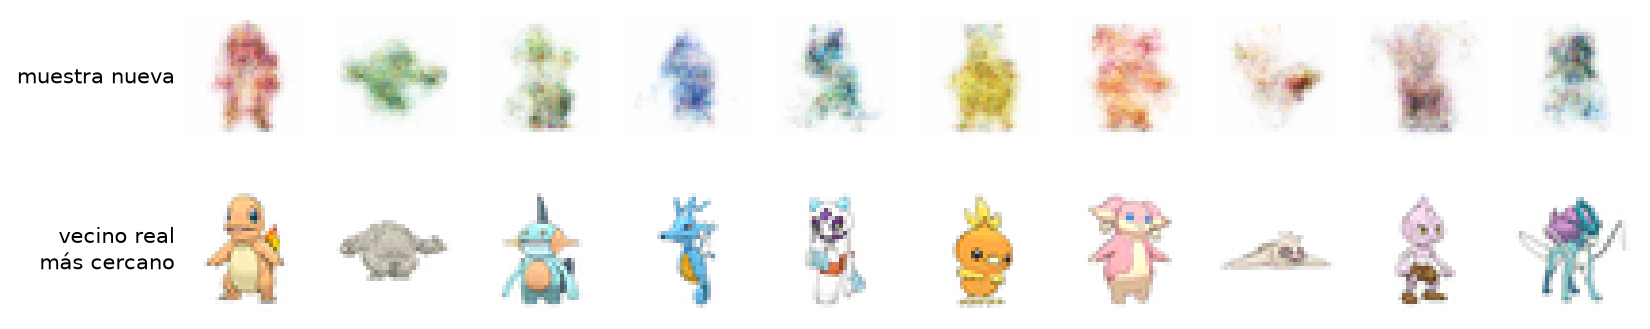
\includegraphics[width=\textwidth]{f_2_nuevas.png}
      \\\fuente{Arriba: muestra elegida y sus tres vecinos reales m\'as cercanos (espacio PCA). Abajo: 10 muestras filtradas y su vecino real.}
    \column{0.45\textwidth}
      \footnotesize
      \begin{block}{Filtro sobre 2000 muestras del prior ($d$=32)}
        (1) no son casi copias; (2) \'area y contraste de la figura entre los percentiles 10 y 90 de los sprites reales. Quedan \textbf{629}.
      \end{block}
      \begin{block}{Argumentos de pertenencia}
        \begin{itemize}
          \item En p\'ixeles: vecino a 6,1 (umbral de copia 4,9).
          \item En PCA: vecino a 2,82 (Pok\'emon real no visto, mediana 4,54).
          \item Las 629 filtradas: mediana 4,56 vs.\ 4,54 de los reales.
        \end{itemize}
      \end{block}
      {\tiny El juicio final es humano: se reconoce por silueta y paleta, no por detalles.}
  \end{columns}
\end{frame}

% ====================================================================== 21b
\begin{frame}{Ej.\ 2b: con convoluciones escritas a mano desaparece el ruido de colores}
  \centering
  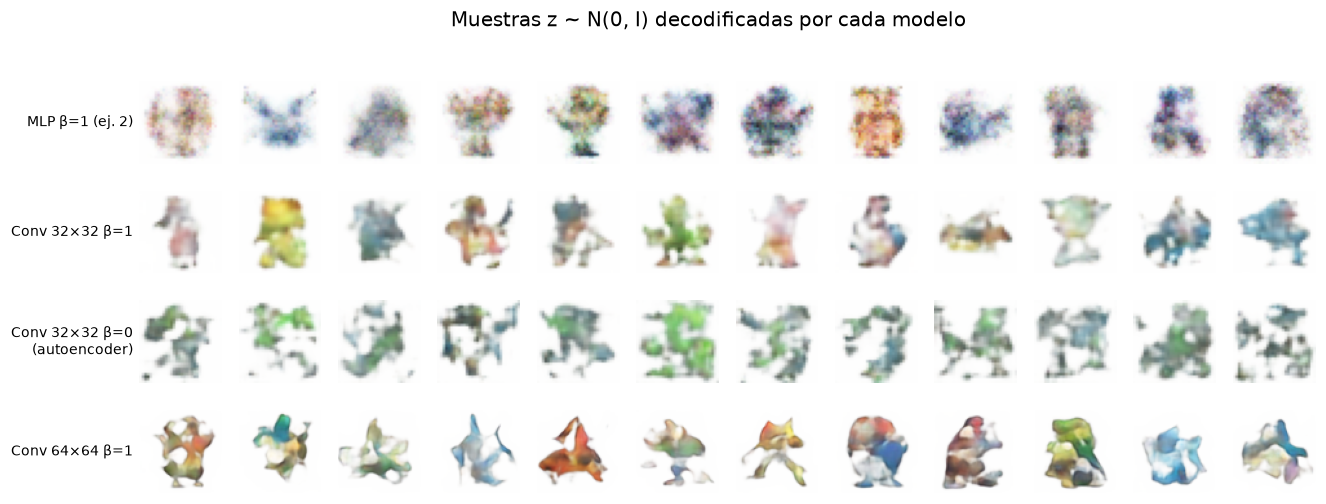
\includegraphics[width=0.88\textwidth,height=0.50\textheight,keepaspectratio]{f_2b_muestras.png}\\[0.1em]
  \begin{columns}[T,onlytextwidth]
    \column{0.23\textwidth}\bignum{5,2}{Fr\'echet, VAE conv. \\ (MLP 6,8; piso 4,1)}
    \column{0.23\textwidth}\bignum{798}{nats en no vistos \\ (MLP 815)}
    \column{0.50\textwidth}\scriptsize\vspace{0.05cm}Mismos datos, p\'erdida, latente y m\'etricas; s\'olo cambian las capas densas por \textbf{convoluciones}, con 7 veces menos par\'ametros. La retropropagaci\'on est\'a escrita a mano (error de gradiente $10^{-8}$); \texttt{cupy} hace las cuentas de arreglos en GPU con la interfaz de \texttt{numpy}. A 64$\times$64 (4 h de GPU) las figuras son m\'as limpias, pero \textbf{siguen sin ojos ni contornos}.
  \end{columns}
\end{frame}

% ====================================================================== 21c
\begin{frame}{Ej.\ 2b: la figura m\'as convincente es el punto medio entre dos Pok\'emon vecinos}
  \begin{columns}[T,onlytextwidth]
    \column{0.60\textwidth}
      \centering
      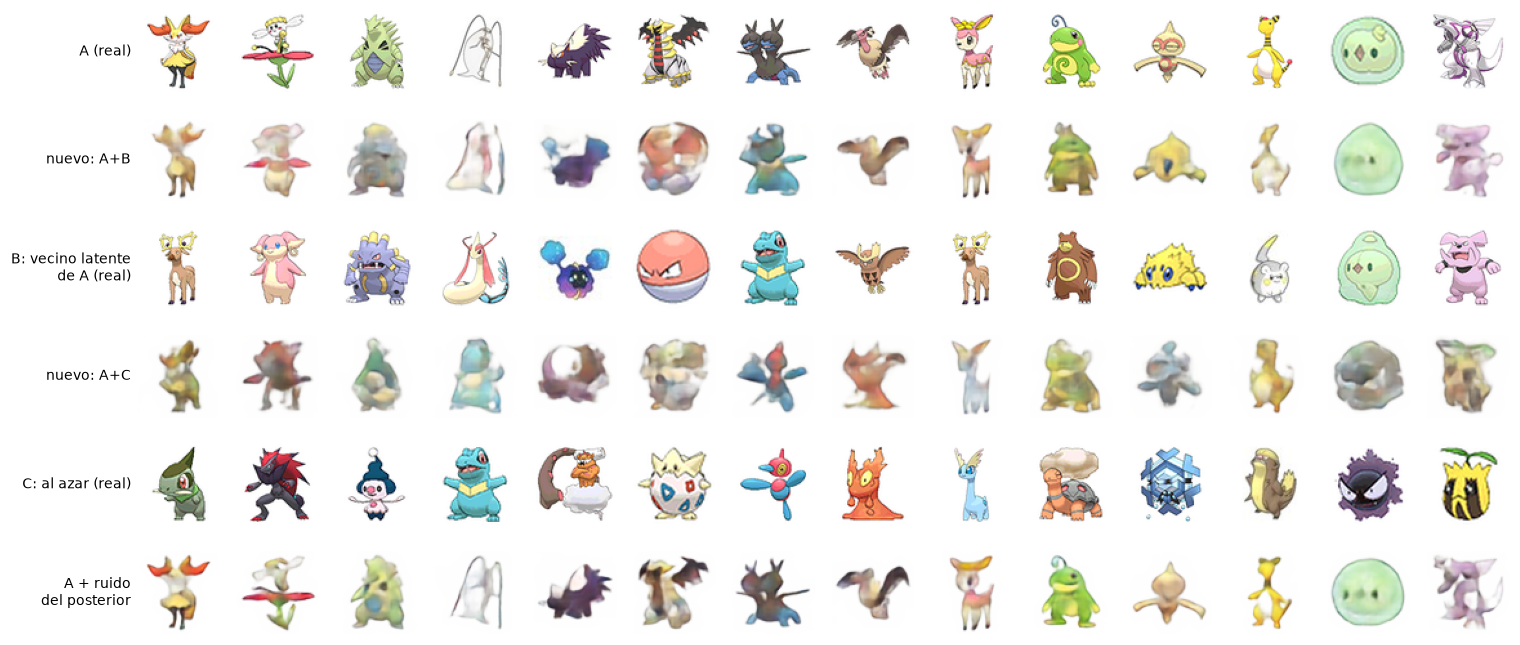
\includegraphics[width=\textwidth,height=0.72\textheight,keepaspectratio]{f_2b_fusiones.png}
      \\\fuente{Modelo convolucional de 64$\times$64. $z=\tfrac12(\mu_A+\mu_B)$; B es el vecino m\'as cercano de A en el espacio latente y C un Pok\'emon al azar.}
    \column{0.37\textwidth}
      \footnotesize
      \begin{block}{Qu\'e muestra}
        \begin{itemize}
          \item \textbf{A+B (vecinos):} criaturas con cuerpo, patas y paleta coherente. 13 de 14 superan el umbral de copia.
          \item \textbf{A+C (al azar):} vuelven a ser manchas.
          \item \textbf{A + ruido del posterior:} casi una copia de A (1 de 14 supera el umbral).
        \end{itemize}
      \end{block}
      \begin{block}{Lectura}
        El decodificador dibuja bien cerca de los c\'odigos que vio. M\'as c\'omputo no agrega detalle: con 728 Pok\'emon distintos el l\'imite son los datos y la verosimilitud por p\'ixel.
      \end{block}
  \end{columns}
\end{frame}

% ====================================================================== 21d
\begin{frame}{Ej.\ 2c: cerca de los datos sale un Pok\'emon nuevo con contorno y ojos}
  \centering
  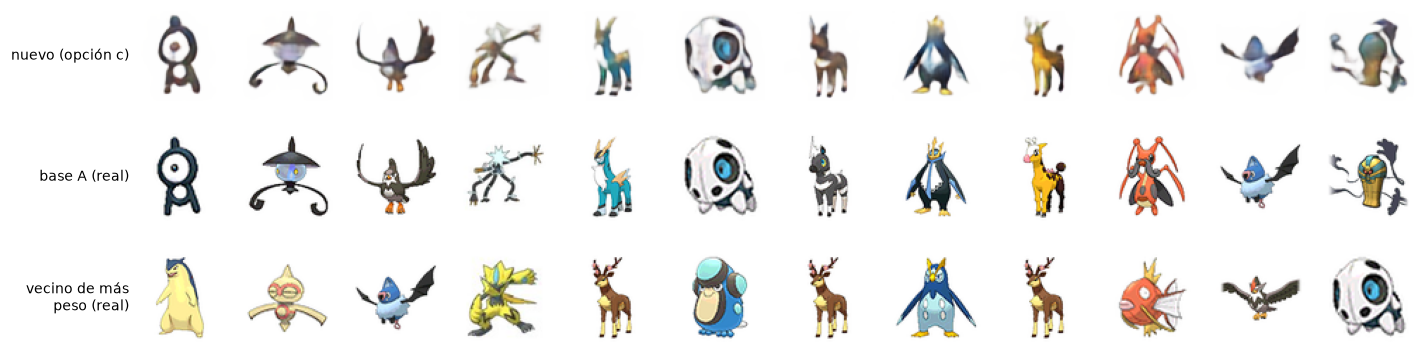
\includegraphics[width=0.90\textwidth,height=0.40\textheight,keepaspectratio]{f_2c_candidatos.png}\\[0.1em]
  \begin{columns}[T,onlytextwidth]
    \column{0.47\textwidth}
      \centering
      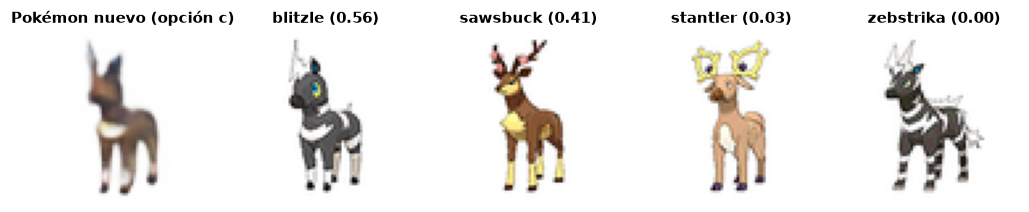
\includegraphics[width=\textwidth,height=0.24\textheight,keepaspectratio]{f_2c_elegida.png}
      \\\fuente{Elegida a ojo entre las 12 m\'as n\'itidas; entre par\'entesis, el peso de cada Pok\'emon en la mezcla.}
    \column{0.50\textwidth}
      \scriptsize
      Modelo del Ej.\ 2b sin reentrenar: $z=w_A\mu_A+\sum_j w_j\mu_{B_j}$, con $A$ un Pok\'emon y $B_j$ sus 3 vecinos latentes.
      \begin{itemize}
        \item \textbf{2022 de 3000} mezclas no son copias (mismo umbral del Ej.\ 2).
        \item Nitidez de las 12 elegidas: \textbf{0,20}, contra 0,11 del prior y 0,25 de un sprite real.
        \item La elegida est\'a a 13,4 del dato m\'as cercano (umbral 11,1).
      \end{itemize}
      \textbf{L\'imite:} es una base deformada hacia sus vecinos, no una especie inventada desde cero.
  \end{columns}
\end{frame}

% ====================================================================== 22
\section{Conclusiones}

\begin{frame}{Conclusiones}
  \footnotesize
  \begin{enumerate}
    \item \textbf{Dos n\'umeros alcanzan para 32 letras, pero hay que encontrarlos}: dos capas ocultas y Adam lo logran en 5/5 semillas (0 px); PCA con 2 componentes deja hasta 15 px.
    \item \textbf{El DAE s\'olo limpia si se entrena con ruido}: un AE sin ruido empeora la entrada; con $d$=8 y $p_{train}$=0,1 deja 0,44 px donde hab\'ia 3,5 (87\,\% menos).
    \item \textbf{El espacio latente de un autoencoder tiene huecos}: reconstruye e interpola entre c\'odigos conocidos, pero no se puede muestrear.
    \item \textbf{El t\'ermino KL es lo que lo vuelve muestreable}: misma red y mismos datos, Fr\'echet 6,8 $\pm$ 0,6 (VAE) contra 19,1 (AE), con piso 4,1. El precio: 815 contra 802 nats de reconstrucci\'on. $\beta$=1 es el equilibrio.
    \item \textbf{Interpolar no prueba que un modelo sea generativo; muestrear del prior s\'i}: entre dos c\'odigos de entrenamiento el AE tambi\'en interpola bien.
    \item \textbf{Parte de la borrosidad era de la MLP, no del VAE} (Ej.\ 2b): con convoluciones el Fr\'echet baja de 6,8 a 5,2 y desaparece el moteado; el detalle fino no aparece muestreando del prior ni con 4 h de GPU, pero s\'i generando cerca de los datos (Ej.\ 2c).
  \end{enumerate}
  \vspace{0.15cm}
  \begin{block}{Relaci\'on entre los ejercicios}
    \scriptsize
    El Ej.\ 1 muestra qu\'e puede hacer la compresi\'on y d\'onde falla (un espacio latente sin estructura); el Ej.\ 2 agrega la estructura estad\'istica que faltaba, reutilizando las mismas capas, el mismo optimizador y la misma p\'erdida de reconstrucci\'on.
  \end{block}
\end{frame}

% ====================================================================== 23
\begin{frame}{Limitaciones, pr\'oximos pasos y reproducibilidad}
  \footnotesize
  \begin{columns}[T,onlytextwidth]
    \column{0.50\textwidth}
      \begin{block}{Limitaciones}
        \begin{itemize}
          \item Ej.\ 1: s\'olo 32 patrones, sin validaci\'on (el enunciado pide representar el conjunto); un \'unico tipo de ruido.
          \item Ej.\ 2 y 2b: muestras \textbf{sin detalle fino} (verosimilitud factorizada por p\'ixel; 728 Pok\'emon, uno de cada uno). El modelo de 64$\times$64 tiene una sola semilla.
          \item Fr\'echet sobre 20 componentes principales: sustituto grueso del FID. El filtro de selecci\'on es una heur\'istica.
          \item 3 semillas por celda y una sola partici\'on de validaci\'on.
        \end{itemize}
      \end{block}
    \column{0.46\textwidth}
      \begin{block}{Pr\'oximos pasos}
        M\'as sprites por Pok\'emon; p\'erdida perceptual o adversaria.
      \end{block}
      \begin{block}{Reproducibilidad}
        \texttt{github.com/yakdudi12/DIAO2A} (carpeta \texttt{TP5}): notebooks, m\'odulos, \texttt{README.md} y \texttt{config.json}. Semillas: 0--4 (Ej.\ 1), 0--2 (Ej.\ 2); modelos finales con semilla 0.
      \end{block}
  \end{columns}
  \vspace{0.25cm}
  \centering\fuente{Bibliograf\'ia: apunte de la c\'atedra (\emph{Artificializando}, cap.\ 18); Goodfellow et al.\ (2016), cap.\ 14; Aggarwal (2023), \S3.4 y \S5.10; Vincent et al.\ (2008); Kingma \& Welling (2014, 2019); Doersch (2016); Higgins et al.\ (2017); Heusel et al.\ (2017).}
\end{frame}

% ======================================================================
\appendix
\section{Anexo}

\figslide{Anexo A: \'epocas hasta $\le 1$ p\'ixel seg\'un el optimizador (35--32--16--2)}{f_1a_epocas.png}{\fuente{Cada punto es una semilla; l\'inea negra = mediana. Rojo = no alcanz\'o $\le$1 p\'ixel en 3000 \'epocas.}}

\begin{frame}{Anexo B: modelo final del Ej.\ 1a, curvas de entrenamiento}
  \centering
  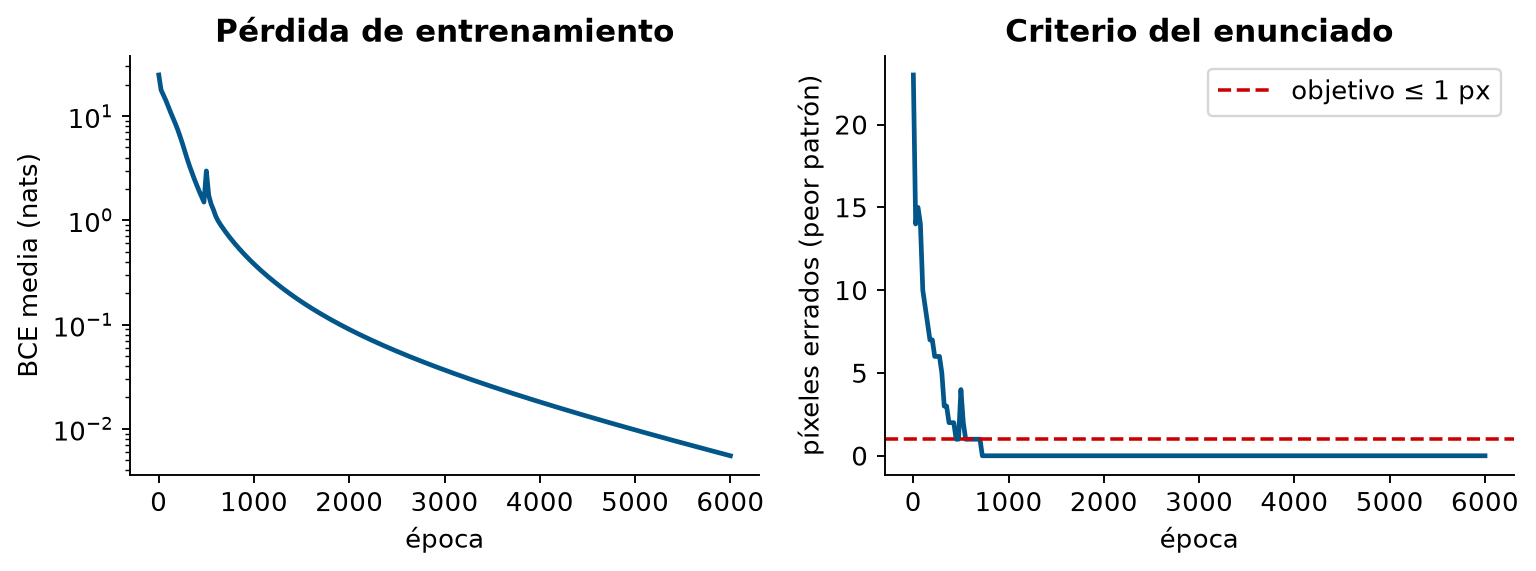
\includegraphics[width=0.9\textwidth,height=0.7\textheight,keepaspectratio]{f_1a_final.png}
\end{frame}

\begin{frame}{Anexo C: interpolaci\'on o $\to$ c en el espacio latente del autoencoder (Ej.\ 1a)}
  \centering
  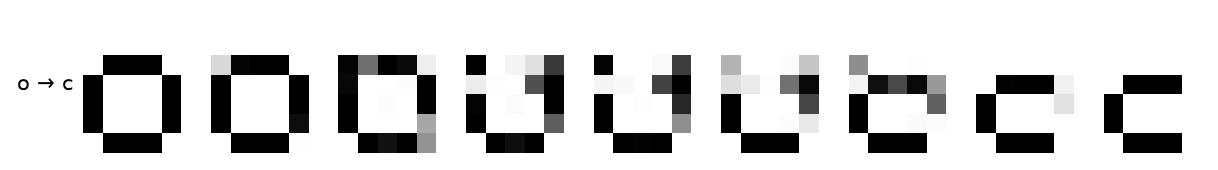
\includegraphics[width=0.85\textwidth,keepaspectratio]{f_1a_interp.png}\\[0.3em]
  {\scriptsize Distancia de Hamming de cada imagen al conjunto de entrenamiento: 0, 0, 2, 5, 6, 4, 1, 0, 0.}
\end{frame}

\figslide{Anexo D: sin KL ($\beta=0$, $d=2$) m\'as c\'odigos quedan fuera del prior y hay regiones dominadas por un solo dato}{f_2_latente_ae.png}{\fuente{Mismo modelo y datos con $\beta=0$. El 74\,\% de los c\'odigos cae en $[-2{,}5;\,2{,}5]^2$ (VAE: 92\,\%). Fr\'echet 109 contra 46 del VAE (semilla 0).}}

\figslide{Anexo E: reconstrucci\'on de Pok\'emon que el modelo nunca vio}{f_2_recon.png}{\fuente{Con $d$=32 se recuperan silueta y paleta, no los detalles. Con $d$=2 queda una mancha del color dominante.}}

\figslide{Anexo F: las interpolaciones son suaves tambi\'en en el autoencoder}{f_2_interp.png}{\fuente{Interpolaci\'on lineal entre las medias $\mu$ de dos Pok\'emon ($d$=32). No distingue los modelos: la diferencia aparece al muestrear del prior.}}

\figslide{Anexo G: \'area y color de las figuras generadas frente a los sprites reales}{f_2_forma.png}{\fuente{2000 muestras por modelo ($d$=32). \'Area media: reales 0,34; VAE 0,46; AE 0,53. El VAE promedia paletas: figuras menos saturadas.}}

\figslide{Anexo H: curvas de entrenamiento del VAE ($\beta=1$, semilla 0)}{f_2_curvas.png}{\fuente{$-$ELBO por imagen en Pok\'emon no vistos (azul) y en el \'ultimo lote de entrenamiento (gris).}}

\end{document}
